\documentclass[preprint,12pt]{elsarticle}
% \documentclass[draft,12pt]{elsarticle}

\usepackage{hyperref}
\usepackage{graphicx}
\usepackage{subcaption}
\usepackage{amssymb}
\usepackage{amsmath}
\usepackage{multirow}
\usepackage{relsize}
\usepackage[utf8]{inputenc}
\usepackage[capitalise]{cleveref}
\usepackage{algorithm}
\usepackage[noend]{algpseudocode}
\usepackage[section]{placeins}
\usepackage{booktabs}
\usepackage{url}

% For the TODOs
\usepackage{xcolor}
\usepackage{xargs}
\usepackage[colorinlistoftodos,textsize=footnotesize]{todonotes}
\newcommand{\todoin}{\todo[inline]}
% from here: https://tex.stackexchange.com/questions/9796/how-to-add-todo-notes
\newcommandx{\unsure}[2][1=]{\todo[linecolor=red,backgroundcolor=red!25,bordercolor=red,#1]{#2}}
\newcommandx{\change}[2][1=]{\todo[linecolor=blue,backgroundcolor=blue!25,bordercolor=blue,#1]{#2}}
\newcommandx{\info}[2][1=]{\todo[linecolor=OliveGreen,backgroundcolor=OliveGreen!25,bordercolor=OliveGreen,#1]{#2}}

%Boldtype for greek symbols
\newcommand{\teng}[1]{\ensuremath{\boldsymbol{#1}}}
\newcommand{\ten}[1]{\ensuremath{\mathbf{#1}}}

\usepackage{lineno}
% \linenumbers

\journal{}

\begin{document}

\begin{frontmatter}

  \title{{DEM}-{SPH} study of particles dispersion in fluid}
  \author[XXX]{Dinesh Adepu\corref{cor1}}
  \ead{d.dinesh@surrey.ac.uk}
  \author[University of Surrey]{Chuan Yu Wu}
  \ead{XXX}
\address[xxx]{xxx}

\cortext[cor1]{Corresponding author}


\begin{abstract}
    Mixing powdered substances in tanks using a stirrer is a common occurrence
    across various industries. Typically, this phenomenon is studied
    numerically due to the complex nonlinear physics involved. In our current
    research, we have developed a solver combining Smoothed Particle
    Hydrodynamics (SPH) and Discrete Element Method (DEM) to investigate the
    mixing behavior of SPH particles within a tank under the influence of a
    stirrer operating at different speeds.  The SPH method governs the fluid
    phase, while the dynamics and interactions of particles are captured by
    the DEM. We achieve a fully resolved coupling between solid particles and
    fluid particles by discretizing solid particles into dummy SPH
    particles. Our validation process includes verifying the fluid solver's
    accuracy through a Poiseuille problem and validating the DEM solver by
    benchmarking interactions between two particles and particle-wall impacts.
    The coupled model's validation extends to various benchmarks, such as
    simulating single-particle entry in both 2D and 3D configurations,
    including a cube entering a tank. Following validation, we proceed with
    the mixing study. We conduct two simulations: one with spherical particles
    of uniform radius and another with particles having varying radius
    distributions.  Our findings reveal that as the stirrer speed increases,
    particles tend to accumulate initially. However, with further increases in
    stirrer speed, particles mix more effectively, and no particle sticking
    occurs. We have leveraged an open-source software, adapting and
    integrating the coupled model to conduct thorough mixing analyses.
\end{abstract}

\begin{keyword}
%% keywords here, in the form: keyword \sep keyword
{particle dispersion}, {particle mixing}, {SPH-DEM}, {stirrer}

%% MSC codes here, in the form: \MSC code \sep code
%% or \MSC[2008] code \sep code (2000 is the default)

\end{keyword}

\end{frontmatter}

% \linenumbers


\FloatBarrier%
\section{Introduction}

Solid–liquid mixing in mechanically agitated vessels is a widely used process
in a multitude of industries, including ore processing, pharmaceuticals and
cosmetics.  Particle agglomeration is found in several parts of industries
involving mixing of particles in a fluid.
\begin{itemize}
\item Nanoparticle fluidization is a process involving to disperse and process
  nanoparticles.  While the nanoparticle agglomerates are
  formed. \cite{liu2016adhesive}.
\item In slurry loop reactors due to the presence of cohesive force between
  the swollen polyethylene (PE) particles. While these PE particles are
  applied in nanotechnology, quantum electronics, optoelectronic, coatings,
  biomedical and information technology. \cite{lu2019experiments}.
  \todo{proposed SJKR}.
\item Systems involving fouling and clogging, such as in heat exchangers,
  ink-jet printing, and catalysis. \cite{trofa2019cfd}.
\item Particle adhesion is of great importance to coating processes due to its
  effect on fluidization.
\item High temperature polymerization fluidized bed reactors
\item Gas-solid fluidized bed reactors are encountered in an extraordinarily
  wide array of chemical, energy and environmental industries due to their
  excellent heat and mass transfer performance. Many gas–solid flows in these
  reactors involve complex interactions between particles such as van der
  Waals forces between small particles (e.g., Geldart types A and C particles,
  and nanoparticles), liquid bridge forces between wet particles,
  electrostatic forces between charged particles, and solid bridge forces
  between molten particles
\item The transport, agglomeration and subsequently deposition of small
  adhesive particles play important roles in many industrial and fundamental
  processes. These processes range from particles accumulating at heat
  transfer surfaces, particles blocking pores in membrane filtration systems,
  particles being inhaled and deposited in our lungs to interstellar medium
  agglomerating causing early stages of new planets to form in space.
\item All agglomeration and deposition processes are a result of particles
  colliding with one another or a wall. The mechanisms governing particle
  collisions of non-adhesive particles in turbulent flows have been devoted
  much attention in literature.
\item \todo{Experimental studies have done involving two particles and small
    scale studies, but they are not sufficient to study or analyse systems
    with bigger scale particles, due to the limitations.}
\item A numerical study is preferred to study a systems like such \cite{xxxx}.
\item While experimental investigation of such processes is often
  impractical due to their highly nonlinear nature, numerical methods offer a
  viable alternative.  While these systems are studied with numerical methods,
  they are a part of two-way coupling models. In numerical method approach,
  one can employ either a mesh-based or meshless technique to study the
  current phenomena.
\end{itemize}


\begin{itemize}
\item The combination of Discrete Element Method (DEM) for solid particle
  interactions and Computational Fluid Dynamics (CFD) for fluid modeling is a
  classic approach in handling particulate flow problem. In mesh-based
  modeling, lattice Boltzmann method (LBM) \cite{xiong2014lbm} and finite
  volume method (FVM) \cite{kloss2012models} are utilized to handle the fluid
  dynamics. Similarly, in meshless schemes like Smoothed Particle
  Hydrodynamics (SPH) \cite{peng2021fully}, Moving Particle Semi-implicit
  (MPS), and Particle Finite Element Method (PFEM) \cite{li2019modeling,
    franci2020pfem}, handles the fluid dynamics.
\item Dispersion of particles by considering the cohseion under the still
  fluid is carried out in \cite{lu2019experiments}. CFD-DEM study is done.
\item We have CFD-DEM study with two fluid model used in this \todo{paper},
  to study the adhesion mixing, fouling.
\item The interaction between the particles is handled using adhesive contact
  models. Such as DMT, JKR \todo{\cite{xxxx}}.
\item The CFD-DEM study is done to study this \todoin{\cite{xxxx}}.
\item The CFD-DEM study is done to study this \todoin{\cite{xxxx}}.
\item An LBM-DEM study is done to study this \todoin{\cite{xxxx}}.
\item An SPH-DEM study with cohesion and without cohesion.\todoin{\cite{xxxx}}.
\end{itemize}


\begin{figure}[!htpb]
  \centering
  \includegraphics[width=0.4\textwidth]{images/hs_tank_fluid_with_particles}
  \caption{An illustrative figure showcasing the dispersion of particles within a free surface tank.}
  \label{intro:schematic}
\end{figure}

\todoin{Rewrite this considering the adhesion. While handling the interaction
  between the fluid and solid particles, the interaction can be categorized
  into a resolved and unresolved coupling. In unresolved coupling, simplified
  models compute forces acting on solid particles within fluid flow,
  \todoin{while fully resolved coupling computes forces comprehensively}. Both
  strategies are applicable in both meshless \cite{cleary2015prediction,
    trujillo2020smooth} and mesh-based \cite{van2008numerical, ma2022review}
  CFD-DEM techniques.  In addition to the study mono-sized particle behaviour
  in a fluid \cite{trujillo2020smooth}, research such as
  \cite{brosh2014accelerating} and \cite{peng2021fully} explore wide particle
  size distributions with CFD-DEM and SPH-DEM respectively.  Regarding
  non-Newtonian fluid modelling in mesh-based schemes, works like
  \cite{li2018dam} are notable and in meshless schemes, \cite{peng2021fully}
  is notable. \citet{zhu2008discrete} and \citet{ma2022review} delve into
  investigations on spherical and non-spherical particles respectively within
  CFD-DEM frameworks.  Meshless CFD-DEM, though fruitful, encounters
  challenges in handling problems with free surfaces and becomes
  computationally demanding with a large number of solid particles, especially
  in fully resolved coupling. In contrast, SPH offers advantages in such
  scenarios due to its inherent capability in handling free surfaces and
  adeptness in modeling large mesh deformation problems, facilitating the
  incorporation of novel physics.}


\todoin{Rewrite this considering the adhesion.

  The SPH method is a meshless numerical method originally proposed by
  \citet{gingold1977smoothed} and \citet{lucy1977numerical} to model
  astrophysics problems. It has been extensively applied to simulate problems
  involving fluids, structural dynamics, fluid-structure interaction, granular
  physics, non-Newtonian fluid flows \cite{peng2021fully} among other areas
  \cite{monaghan2012smoothed}.  Various kind of particulate flows, involving,
  simple spherical particles mixing using unresolved coupling
  \cite{cleary2015prediction, markauskas2019coupled} and with debris flow
  \cite{canelas2016sph} with fully resolved coupling approach were analysed
  using SPH-DEM.  Handling particles of arbitrary shape in fluid flow is
  addressed in various works, including those by \citet{peng2021fully,
    canelas2016sph, amicarelli2015smoothed}.  Several variants of SPH, such as
  WCSPH \cite{peng2021fully, cleary2015prediction}, and ISPH
  \cite{asai2021fluid}, are utilized for modeling fluid flow with particulate
  flows. The coupling between fluid and rigid bodies in the fully resolved
  category employs techniques such as the fixed ghost particle technique
  \cite{canelas2016sph, asai2021fluid}, single layers of dummy SPH particles
  \cite{peng2021fully}, and simple repulsive forces
  \cite{monaghan2009sph}. Coupling between SPH fluid particles and solid
  structures discretized as vertex edges is also proposed by
  \citet{park2023new}. Particle settling with variable sizes is studied by
  \citet{zou2022study}.  Elastic behavior of spherical particles and
  dispersion studies are conducted by \citet{ng2021numerical}.  Interaction
  between rigid bodies of arbitrary sizes is addressed using various
  techniques, such as those discussed in papers by \citet{asai2021fluid},
  \citet{peng2021fully}, \citet{canelas2016sph}.}



\todoin{Current research gap}.
\todoin{
  \begin{itemize}
  \item A detailed study of two particles settling in a tank is studied in
    several studies. Here no adhesion among the particles is studied.
  \item LBM-DEM has recently studied this, with particles settling in tank
    considered cohesion.
  \item A clear understanding of simple systems settling in tank with give us
    more understanding of how dipserison in a system works.
  \item In that line, in a recent study, two particles settling with different
    radius size without cohesion involved has been studied in \cite{xxxx} paper.
  \item To understand the dispersion of particles involving cohesion, in the
    current work, we study the behaviour of two particles settling with
    different diameter ratios, which are placed a distance apart.
  \item We consider DMT model to handle the cohesion among the particles.
  \item We will use the DKT tests of \cite{chen2021numerical}, which is
    LBM-DEM coupled problem.
  \item Finally a mixing analysis of several particle with cohesion involved
    is studied.
  \end{itemize}
}.
\todoin{
  \begin{itemize}
  \item A single particle settling in the tank.
  \item A DKT without cohesion as a benchmark
  \item Two particles with different radius settling under gravity.
  \end{itemize}
}.
Upon confirming the fidelity of the solver, we proceed with analyzing the
mixing behavior of various spherical particles influenced by a stirrer in a
tank. We investigate scenarios involving particles of different densities,
stirrer velocities, and variable sizes as part of our case study. The
development work is conducted using PySPH\cite{ramachandran2021pysph}, an
open-source code available at \url{https://github.com/pypr/pysph}.  We modify
the current codebase to integrate implementations of the Discrete Element
Method (DEM) and the Smoothed Particle Hydrodynamics (SPH) coupled with DEM
model for our ongoing research. To ensure reproducibility, we utilize the
automan package \cite{ramachandran2018automan} to automate all results
generated in the current manuscript, aiming for a reproducible research
approach.



The structure of this paper is as follows: In
\cref{sec:fluid-modeling}, we explain the numerical method used to model fluid
dynamics. \Cref{sec:rbd} outlines the equations governing the dynamics
of rigid bodies and the contact force model employed to resolve collisions
among them. The coupling between rigid spherical particles and the fluid is
detailed in \cref{sec:rfc}. Our results are presented in
\cref{sec:results}, where various problems from the literature are simulated to
validate the current solver, and particle dispersion is examined.



\FloatBarrier%
\section{Fluid modeling}
\label{sec:fluid-modeling}
In the current work, we follow a weakly-compressible SPH approach to model the
fluid. The continuum in SPH is modeled using particles, which has physical
properties such as mass, velocity, and these particles interact based on the
governing equations using a Guassian-like kernel
\cite{monaghan-review:2005,morris1997modeling}.


\FloatBarrier%
\subsection{Fluid governing equations}
\label{sec:fluid--governing-equations}
The fluid motion is governed by the conservation of mass and the conservation
of linear momentum, which can be expressed by the following equations:
\begin{equation}
  \label{eq:ce}
  \frac{d \rho}{d t} = - \rho \; \frac{\partial u_i}{\partial x_i},
\end{equation}
\begin{equation}
  \label{eq:me}
  \frac{d u_i}{d t} = \frac{1}{\rho} \; \frac{\partial \sigma_{ij}}{\partial x_j}
  + g_i,
\end{equation}
where $\rho$ is the density, $u_i$ is the $i$\textsuperscript{th} component of
the velocity field, $x_j$ is the $j$\textsuperscript{th} component of the
position vector, $g_i$ is the component of body force per unit mass and
$\sigma_{ij}$ is stress tensor.

The stress tensor is split into pressure and viscous parts,
\begin{equation}
  \label{eq:fluid-stress-decomposition}
  \sigma_{ij} = - p \delta_{ij} + 2 \eta \frac{\partial u_i}{\partial x_j}
\end{equation}
where $\eta$ is the kinematic viscosity of the fluid, $p$ is the pressure,
$\delta_{ij}$ is the Kronecker delta function.


\FloatBarrier%
\subsection{Discretized fluid governing equations}
\label{sec:sph--governing-equations}
The governing equations involve function, derivative and divergence
operators. In SPH, these operators are approximated based on the positions,
mass and the kernel values of the discretized particles. Assume that the
domain is discretized into N particles with mass $m_i$ and volume
$V_i$, We have
\begin{equation}
  \label{eq:mass_repr}
  m_j = V_i \> \rho_i.
\end{equation}
Based on this discretization, the discrete function approximation is given as,
\begin{equation}
  \label{eq:discrete_form}
  A_i = \sum_{j \in \text{Neigh}(i)}\> \frac{m_j}{\rho_j} A_j\> W(\ten{x}_i - \ten{x}_j, h),
\end{equation}
where $A(\boldsymbol{x}_i) = A_i$ is the value of the field property of
particle i, similarly for $A_j$. Here, $\text{Neigh}(i)$ is the neighbours of
particle $i$.  A symmetric derivative approximation~\cite{Violeau16} is given
as,
\begin{equation}
  \nabla A(\ten{x}_i) = \rho_i \sum_{j} m_j \left(\frac{A_i}{\rho_i^2} + \frac{A_j}{\rho_j^2}\right) \nabla W_{ij}.
\end{equation}
A symmetric gradient operator ensures equal and opposite forces acting on the
particles.


An approximation of the divergence operator is used to discretize the
\cref{eq:ce}.  It is given as,
\begin{equation}
  \label{intro:eq:sph-continu-div-final}
  \nabla \cdot \ten{v}(\ten{x}_i) = \frac{1}{\rho_i} \sum_{j} m_j \left(\ten{v}_j - \ten{v}_i\right) \cdot \nabla W_{ij}.
\end{equation}


% \subsection{Discretized fluid governing equations}
The SPH discretization of the continuity
equation~\cref{eq:sph-discretization-continuity} is given as,
\begin{equation}
  \label{eq:sph-discretization-continuity}
  \frac{{d}\rho_a}{dt} = \sum_{b} \; \frac{m_b}{\rho_{b}} \;
  \rho_{a} \; {\ten{u}}_{ab} \; \cdot \nabla_{a} W_{ab},
\end{equation}

%
Similarly, the discretized momentum equation is written as,
\begin{multline}
  \label{eq:sph-momentum-fluid}
  \frac{{d}\ten{u}_{a}}{dt} = - \sum_{b} m_b
  \bigg(\frac{p_a}{\rho_a^2} + \frac{p_b}{\rho_b^2}\bigg)
  \nabla_{a} W_{ab}
 \;+\;
  \sum_{b} m_b \frac{4 \eta \nabla W_{ab}\cdot
    \ten{r}_{ab}}{(\rho_a + \rho_b) (r_{ab}^2 + 0.01 h_{ab}^2)} \ten{u}_{ab}  \;+\;
  \ten{g}_{a},
\end{multline}
where $\ten{I}$ is the identity matrix, $\eta$ is the kinematic viscosity of the
fluid and \todoin{\cite{morris1997modeling}} formulation is used to discretize the
viscosity term.

We add to the momentum equation an additional artificial viscosity term
$\Pi_{ab}$~\cite{monaghan-review:2005} to maintain the stability of the
numerical scheme, given as,
\begin{align}
  \label{eq:mom-av}
  \Pi_{ab} =
  \begin{cases}
\frac{-\alpha h_{ab} \bar{c}_{ab} \phi_{ab}}{\bar{\rho}_{ab}}
  & \ten{u}_{ab}\cdot \ten{r}_{ab} < 0, \\
  0 & \ten{u}_{ab}\cdot \ten{r}_{ab} \ge 0,
\end{cases}
\end{align}
where,
%
\begin{equation}
  \label{eq:av-phiij}
  \phi_{ab} = \frac{\ten{u}_{ab} \cdot \ten{r}_{ab}}{r^2_{ab} + 0.01 h^2_{ab}},
\end{equation}
%
where $\ten{r}_{ab} = \ten{r}_a - \ten{r}_b$,
$\ten{u}_{ab} = \ten{u}_a - \ten{u}_b$, $h_{ab} = (h_a + h_b)/2$,
$\bar{\rho}_{ab} = (\rho_a + \rho_b)/2$, $\bar{c}_{ab} = (c_a + c_b) / 2$, and
$\alpha$ is the artificial viscosity parameter.  The pressure $p_a$ is evaluated
using an equation of state:
\begin{equation}
\label{eqn:sph-eos}
  p_a = K \bigg(\frac{\rho_a}{\rho_{0}} - 1 \bigg).
\end{equation}
Where, $K=\rho_0 \, c_0^2$ is bulk modulus of the body, with
$c_0=10 \times V_{\text{max}}$ is speed of sound, while $\rho_0$ as the
initial density of the particles.


\FloatBarrier%
\subsection{Boundary Conditions}
\label{sec:boundary_conditions}

The ghost particle approach proposed by \citet{Adami2012} is used to model the
boundaries. We use three layers of ghost particles to model the solid wall.
The properties of the solid wall are interpolated from the fluid particles.

When the viscous force is computed, the no slip boundary condition is used,
where the velocity on the boundary set as,
\begin{equation}
  \label{eq:no-slip-bc-u}
  \ten{u}_{\text{Ga}} = 2 \ten{u}_{\text{p}} - \ten{\hat{u}}_{\text{a}}.
\end{equation}
The projected velocity $\ten{\hat{u}}_{\text{a}}$ on the ghost particles is
computed using,
\begin{equation}
  \label{eq:v-ghost}
  \ten{\hat{u}}_a = \frac{\sum_b\ten{u}_b W_{ab}}{\sum_b W_{ab}},
\end{equation}
where $\ten{u}_b$, is the velocity of the fluid particle $b$ and $W_{ab}$ is the kernel
value between the fluid particle and the ghost particle.


The pressure of the boundary particle is extrapolated from its surrounding
fluid particles by the following equation,
\begin{equation}
  \label{eq:pressure-bc}
  p_w = \frac{\Sigma_f p_f W_{wf} + (\ten{g} - \ten{a}_{\ten{w}}) \cdot \Sigma_f
    \rho_f \ten{r}_{wf} W_{wf}}{\Sigma_f W_{wf}},
\end{equation}
where $\ten{a}_w$ is the acceleration of the wall. The subscript $f$ denotes
the fluid particles and $w$ denotes the wall particles.



\FloatBarrier%
\section{Rigid body dynamics}
\label{sec:rbd}
% The rigid body is discretized into particles with equal spacing each particle
% with mass $m_i$ and density $\rho_i$. Rigid body has a total 6 degrees of
% freedom (DOF), divided into $3$ translational and $3$ rotational.

% An approach using quaternions is given in \cite{dietemann2020smoothed}
% An another paper using quaternions \cite{guan2024numerical}


The equations governing the dynamics of a rigid body are, balance of linear and
angular momentum given by,
\begin{equation}
  \label{eq:rfc:balance_linear_mom}
  \frac{d \; (M \ten{v}_{cm})}{d t} = \sum_i \ten{F}_i,
\end{equation}
\begin{equation}
  \label{eq:rfc:balance_angular_mom}
  \frac{d \ten{L}}{d t} = \teng{\tau}_{cm},
\end{equation}
where $M$, $\ten{v}_{cm}$ are the mass and velocity of the center of mass of the rigid body.
$\ten{F}_i, \teng{\tau}_{cm}, \ten{L} $ are force acting at point $i$, torque and
angular momentum about the center of mass of the rigid body. In the current
case, force acting on the particle $i$, $\ten{F}_i$, is due to the interaction
with the other bodies and with the fluid particles, and any other body forces.
The torque $\teng{\tau}_{cm}$ and angular momentum $\ten{L}$ are computed as,
\begin{equation}
  \label{eq:rfc:torque}
 \teng{\tau}_{cm} = \sum_i \ten{F}_i \times (\ten{x}_{cm} - \ten{x}_{i}),
\end{equation}
\begin{equation}
  \label{eq:rfc:moi}
  \teng{L} =
  \sum_i \; \ten{r}_i \times \; (\teng{\omega} \times \ten{r}_i)
  = \sum_i \; m_i \; [(\ten{r}_i \cdot \ten{r}_i) \ten{I} - \ten{r}_i \otimes \ten{r}_i].
\end{equation}
Here $\ten{x}_{cm}$ and $\omega$ are the position of the center of mass and
angular velocity of the rigid body. $m_i$, $\ten{x}_{i}$, $\ten{r}_i$ are the
mass, position of particle, and position of particle $i$ with respect to vector
center of mass.

\begin{figure}[!htpb]
  \centering
  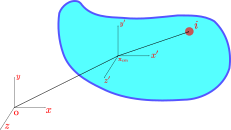
\includegraphics[width=0.7\textwidth]{images/rigid_body/rigid_body}
  \caption{Body frame and local frame description of rigid body}
  \label{fig:gloabl_body_frame_rb}
\end{figure}
We use two coordinate frames to capture the dynamics of the rigid body, a
global frame and a body frame as shown in
\cref{fig:gloabl_body_frame_rb}. The body fixed frame, which moves with
rigid body is always located at the center of mass ($\ten{x}_{cm}$). The
state of the rigid body at a given time ($t$) can be described using position
($\ten{x}_{cm}$) and velocity ($\ten{v}_{cm}$) of the center of mass, a
rotation matrix($\ten{R}$) to represent the orientation of the rigid body with
respect to the global frame, and angular velocity($\teng{\omega}$). The center
of mass is computed as
\begin{equation}
  \label{eq:rfc:center_of_mass}
  \ten{x}_{cm} = \frac{\sum_i m_i \; \ten{x}_{i} }{\sum_i m_i }.
\end{equation}
The position of the discretized particle ($i$) in
\cref{fig:gloabl_body_frame_rb} belonging to the rigid body at time $t$ can be
computed as,
\begin{equation}
  \label{eq:rfc:rb_particle_pos_update}
  \ten{x}_i = \ten{x}_{cm} + \ten{r}_{i},
\end{equation}
with
\begin{equation}
  \label{eq:rfc:rb_particle_pos_update}
  \ten{r}_i = \ten{R} \overline{\ten{r}}_{i}.
\end{equation}
Here $\overline{\ten{r}}_{i}$ is the position of the particle $i$ about the body
frame axis and remains constant through out the simulation. The rotation matrix
$\ten{R}$ is used to bring the body frame position vector to the global frame
$\ten{O}$. Similarly the velocity vector is computed as,
\begin{equation}
  \label{eq:rfc:rb_particle_vel_update}
  \ten{v}_i = \ten{v}_{cm} + \teng{\omega} \times \ten{r}_{i}.
\end{equation}

We evolve the state of the rigid body through the integration of the
\cref{eq:rfc:balance_linear_mom,eq:rfc:balance_angular_mom}. The linear velocity of the
center of mass ($\ten{v}_{cm}$) and angular momentum ($\ten{L}$) at the next
timestep are computed as,
\begin{equation}
  \label{eq:rfc:lin_vel_cm_update}
  \ten{v}_{cm}^{n+1} = \ten{v}_{cm}^{n} + \frac{\ten{F}_{cm}}{M} \; \Delta t,
\end{equation}
\begin{equation}
  \label{eq:rfc:ang_mom_update}
  \ten{L}^{n+1} = \ten{L}^{n} + \teng{\tau}_{cm} \; \Delta t.
\end{equation}
Here, $\ten{F}_{cm} = \sum_i \ten{F}_i$.

The position of the center of mass and the rotation matrix ($\ten{R}$) are updated
by,
\begin{equation}
  \label{eq:rfc:lin_pos_cm_update}
  \ten{x}_{cm}^{n+1} = \ten{x}_{cm}^{n} + \ten{v}_{cm}^{n} \; \Delta t,\\
  \ten{R}^{n+1} = \ten{R}^{n} + \tilde{\teng{\omega}}^{n} \, \ten{R}^{n} \; \Delta t,
\end{equation}
where $\tilde{\teng{\omega}}^{n}$ is matrix formulation of angular velocity
$\omega$. The angular velocity at the new time step is computed with
\begin{equation}
  \label{eq:rfc:ang_velocity_update}
  \teng{\omega}^{n+1} = (\textit{\teng{I}}^{-1})^{n+1} \; \ten{L}^{n+1}.
\end{equation}
Here, moment of inertia at the new time step is computed as,
\begin{equation}
  \label{eq:rfc:moi_update}
  (\textit{\teng{I}}^{-1})^{n+1} = \ten{R}^{n+1} \textit{\teng{\overline{I}}}^{-1} (\ten{R}^{n+1})^T.
\end{equation}
where moment of inertia ($\textit{\teng{\overline{I}}}^{-1}$) in body frame is
used to compute in global frame at every time instant for faster computations.
The moment of inertia ($\textit{\teng{\overline{I}}}$) is computed as,
\begin{equation*}
\textit{\teng{\overline{I}}} =
\begin{bmatrix}
\sum_i m_i (y_i^2 + z_i^2) & -\sum_i m_i x_iy_i & -\sum_i m_i x_iz_i\\
-\sum_i m_i x_iy_i & \sum_i m_i (x_i^2 + z_i^2) &  -\sum_i m_i y_iz_i\\
-\sum_i m_i  x_iz_i & -\sum_i m_i y_iz_i & \sum_i m_i (x_i^2 + y_i^2)
\end{bmatrix}.
\end{equation*}

The position and velocity of the particles of the rigid body are updated by
\begin{eqnarray}
  \label{eq:rfc:rb_particle_pos_update}
  \ten{r}_i = \ten{R} \cdot \overline{\ten{r}}_{i},\\
  \ten{x}_i = \ten{x}_{cm} + \ten{r}_{i},\\
  \ten{v}_i = \ten{v}_{cm} + \teng{\omega} \times \ten{r}_{i}.
\end{eqnarray}

The force acting on particle $i$ is composed of interaction with the other rigid
bodies, and the fluid, given as
\begin{eqnarray}
  \label{eq:rfc:rb_particle_pos_update}
  \ten{F}_i = \ten{F}_{\text{Fl}}^i + \ten{F}_{\text{cont}}^i
\end{eqnarray}
We follow \cref{sec:dem} to compute force
$\ten{F}_{\text{cont}}^a$ acting on particle $i$ due to the interaction with
the rigid bodies. The force $\ten{F}_{\text{rfc}}^i$ acting due to the
interaction with the fluid particles follows \cref{sec:rfc}.



\FloatBarrier%
\subsection{Contact models}
\label{sec:dem}

\begin{figure}[!htpb]
  \centering
  \includegraphics[width=0.7\textwidth]{images/spherical_particles_dem_representation}
  \caption{Demonstration of contact handling between two rigid spherical
    particles immersed in a fluid tank.}
  \label{fig:spherical-particles-in-tank-dem}
\end{figure}

We resolve the contact among the spherical particles using the discrete
element method \cite{luding_dem_2008}. In the current work we have utilized a
non-linear contact force model. In DEM, the force acting on a particle $a$ due
to the interaction with the particle $b$ is resolved into a normal and
tangential component. The normal force component represents a repulsive force,
while the tangential component is used to model the friction between the
interacting particles.  The normal force ($\teng{F}_a^{n}$) on particle $a$
due to the interaction with the particles $b$ is given by a non-linear,
Hetzian model \cite{brilliantov1996model},
\begin{equation}
  \label{eq:contact-algorithm-normal}
  \ten{F}_a^n = k_n \delta_{n} \ten{n}.
\end{equation}
Here, the overlap $\delta_{n}$ is computed using
\begin{equation}
  \label{eq:cf-overlap}
  \delta_{n} = R_{a} + R_{b} - r_{ab},
\end{equation}
$k_r$ is the normal spring stiffness coefficient, which is computed using the
material properties of the bodies in contact, given by:
\begin{equation}
  \label{eq:kf-stiffness}
  k_n = \frac{4}{3} \; E^{*} \; \sqrt{R^{*} \delta_n}
\end{equation}
\begin{equation}
  \label{eq:kf-stiffness}
  k_t = 8 \; G^{*} \; \sqrt{R^{*} \delta_n}
\end{equation}

\begin{equation}
  \label{eq:kf-stiffness}
  \eta_n = -2 \sqrt{\frac{5}{6}} \beta \; \sqrt{S_n m^*}
\end{equation}
\begin{equation}
  \label{eq:kf-stiffness}
  \eta_t = -2 \sqrt{\frac{5}{6}} \beta \; \sqrt{S_t m^*}
\end{equation}

\begin{equation}
  \label{eq:kf-stiffness}
  S_n = 2 E^{*} \sqrt{R^{*} \delta_n}
\end{equation}
\begin{equation}
  \label{eq:kf-stiffness}
  S_t = 8 G^{*} \sqrt{R^{*} \delta_n}
\end{equation}




$\frac{1}{E^{*}} = \frac{1 -\nu_a^2}{E_a} + \frac{1 -\nu_b^2}{E_b}$
$\frac{1}{G^{*}} = \frac{2 (2 - \nu_a) (1 + \nu_a)}{E_a} +  \frac{2 (2 - \nu_b) (1 + \nu_b)}{E_b}$
$\beta = \frac{\ln{e}}{\ln{e}^2 + \pi}$
$R^{*} = \frac{R_a R_b}{R_a + R_b}$



\subsection{Tangential force computation}
\label{sec:tangential-force-computation}
To handle the frictional contact, we associate a tangential spring attached to
particle $a$ and particle $b$ to compute the tangential force, which initially has
a magnitude of zero ($|\Delta \textit{\textbf{l}}_a|=0$). The tangential spring
is activated when the particle comes into contact with particle $b$. The
tangential force is history-dependent. The contact friction force is
proportional to the tangential displacement, which is integrated over
the contact time as
\begin{equation}
  \label{eq:tangential-force}
  \ten{F}_{a}^{t^{n+1}} =
  -k_f \Delta \textit{\textbf{l}}_a^{\,n + 1} =
  -k_f \big[\big(\Delta {\textit{\textbf{l}}}_a^{\,n} \
  + \ten{v}_{ab}^{n + 1} \Delta t\big) \cdot \ten{t}_a^{n + 1} \big] \
  \ten{t}_a^{n + 1},
\end{equation}
where $\Delta t$ is the time step, $\ten{v}_{ab} = \ten{v}_{a} - \ten{v}_b$ is the
relative velocity of particle $a$ with respect to the contacting particle $b$,
and $k_f$ is the tangential spring stiffness coefficient. The tangential
spring stiffness is computed similar to the normal spring
stiffness\cite{golshan2023lethe}.  The tangential unit vector is computed by,
\begin{equation}
  \label{eq:tangential-vect}
  \ten{t}_a = \frac{\ten{v}_{ab} - (\ten{v}_{ab} \cdot \ten{n}) \ten{n}}{|\ten{v}_{ab} - (\ten{v}_{ab} \cdot \ten{n}) \ten{n}|}.
\end{equation}

The tangential force is coupled to the normal force through the Coulomb's law,
\begin{equation}
  \label{eq:Coulomb-law}
  \ten{F}_{a}^{t} = \min(\mu |\ten{F}_{a}^{n}|, |\ten{F}_{a}^{t}|) \
  \frac{\ten{F}_{a}^{t}}{|\ten{F}_{a}^{t}|}.
\end{equation}
This allows us to impose the sliding friction condition between the
interacting solids. Finally, the total force acting on the particle $a$ due to
the interaction with particle $b$ is:
\begin{equation}
  \label{eq:contact-force}
  \ten{F}_{a}^{\text{cont}} = \ten{F}_{a}^{n} + \ten{F}_{a}^{t}
\end{equation}

An equal and opposite force of the same magnitude is applied to
particle $b$, given as
\begin{equation}
  \label{eq:contact-force}
  \ten{F}_{b}^{\text{cont}} = - \ten{F}_{a}^{\text{cont}}.
\end{equation}



\FloatBarrier%
\section{Rigid fluid coupling}
\label{sec:rfc}

% Coupling equation with single particles he2017coupled
% Coupling with dummy particles \cite{guan2024numerical}
% A different coupling equation meng2022hydroelastic

\begin{figure}[!htpb]
  \centering
  \begin{subfigure}{0.22\textwidth}
    \centering
    \includegraphics[width=1.0\textwidth]{images/rfc_explantion_schematic/real_spherical_particles}
    \subcaption{A rigid spherical particle}%\label{fig:rings:ipst-nu-0.47-0}
  \end{subfigure}\hspace{15mm}%
  \begin{subfigure}{0.24\textwidth}
    \centering
    \includegraphics[width=1.0\textwidth]{images/rfc_explantion_schematic/sph_sampled_spherical_particles}
    \subcaption{A rigid spherical particle sampled with dummy SPH particles}%\label{fig:rings:ipst-nu-0.47-1}
  \end{subfigure}
  \caption{}
\label{fig:real_particle_sph_sampling}
\end{figure}
To calculate the force exerted on the spherical particle by the surrounding
fluid, we employ a method involving the sampling of the spherical particle
using dummy Smoothed Particle Hydrodynamics (SPH) particles, depicted in
\cref{fig:real_particle_sph_sampling}. These SPH particles are evenly
distributed and remain stationary, moving in tandem with the velocity of the
rigid particle at any given location. To establish the pressure of these SPH
particles, we utilize the fixed ghost particle boundary technique outlined in
\cref{sec:boundary_conditions}.



With spherical particles being discretized into SPH particles and immersed in
fluid can be seen in \cref{fig:many_rb_in_fluid_sph_particles}.
\begin{figure}[!htpb]
  \centering
  \includegraphics[width=0.7\textwidth]{images/rfc_zoomed_combined}
  \caption{A rigid spherical particle sampled with dummy SPH particles being
    immersed in a fluid tank. An SPH particle representation}
  \label{fig:many_rb_in_fluid_sph_particles}
\end{figure}
The force on the fluid particle due to the
interaction with the sampled dummy SPH particles is considered in the momentum
\cref{eq:sph-momentum-fluid} and the continuity
\cref{eq:sph-discretization-continuity}. The force acting on the sampled dummy
SPH particle due to the interaction with the fluid is given by,
\begin{equation}
  \label{eq:rfc-force}
  \ten{F}_{\text{rfc}}^a = -m_a \sum_{f} m_f \bigg(\frac{p_f}{\rho_{f}^2} +
  \frac{p_a}{\rho_{a}^2}\bigg) \nabla_{a} W(x_{af}),
\end{equation}
where, $m_a$ signifies the hydrodynamic mass of the sampled dummy SPH particle,
and $\rho_a$ represents its hydrodynamic density. While $m_f$, $p_f$ and
$\rho_f$ are mass, pressure and density of the fluid particle.


\FloatBarrier%
\section{Time Integration}

We use the kick-drift-kick scheme \cite{monaghan-review:2005} for the time integration. We move the
velocities of the fluid and the solid particles to half time step,
\begin{equation}
  \label{eq:velocity-update-stage-1}
  \ten{u}_a^{t+\frac{1}{2} \Delta t} = \ten{u}_a^{t} + \frac{\Delta t}{2} \bigg(\frac{d\ten{u}_{a}}{dt}\bigg)^t,
\end{equation}
here, $()_a^t$ represents the properties of particle $a$ at time $t$ and
$()_a^{t+\frac{1}{2} \Delta t}$ corresponds to the halfway point between time
$t$ and $t + \Delta t$. Then the time derivative of density is calculated using the
\cref{eq:sph-discretization-continuity}, with velocities at half time step
employed for the calculation.  The updated density and particle position for
the new time step are determined by,
\begin{equation}
  \label{eq:density-update-stage-2}
  \rho_{a}^{t+\Delta t} = \rho_{a}^{t} + \Delta t \; \bigg(\frac{d\rho_{a}}{dt}\bigg)^{t+\frac{1}{2} \Delta t},
\end{equation}
\begin{equation}
  \label{eq:position-update-stage-2}
  \ten{r}_{a}^{t+\Delta t} = \ten{r}_{a}^{t} + \Delta t \; \ten{u}_{a}^{t+\Delta t}.
\end{equation}
%
Finally, at new time-step particle position, the momentum velocity is updated
\begin{equation}
  \label{eq:velocity-update-stage-3}
  \ten{u}_a^{t+\Delta t} = \ten{u}_a^{t+\frac{1}{2}\Delta t} + \frac{\Delta t}{2} \bigg(\frac{d\ten{u}_{a}}{dt}\bigg)^{t+\Delta t}.
\end{equation}


The modeling of rigid-rigid interaction requires a smaller time step than the
fluid. We choose the minimum of these two timesteps to move the system forward
in time. For the numerical stability of fluid, the time step depends on the
Courant–Friedrichs–Lewy (CFL) condition \cite{monaghan-review:2005} as,
\begin{equation}
  \label{eq:rfc:time-step-cfl}
  \Delta t_{\text{fluid}} = \mathrm{min} \bigg( 0.25 \; \frac{h}{c + |U|} ,  0.25 \; \frac{h^2}{\nu},  0.25 \; \frac{h^2}{g} \bigg),
\end{equation}
where $|U|$ is the maximum velocity magnitude, $c$ is the speed of sound
typically chosen as $10 |U|$ for fluids in this work. For rigid body, the time
step is constrained \cite{cundall_discrete_1979} as,
\begin{equation}
  \label{eq:rfc:time-step-body-force}
  \Delta t_{\text{rb}} \leq \frac{\pi}{50} \sqrt{\frac{m}{k_r}}.
\end{equation}
A minimum timestep is chosen as
\begin{equation}
  \label{eq:rfc:time-step-body-force}
  \Delta t = min(\Delta t_{\text{fluid}}, \Delta t_{\text{rb}}).
\end{equation}





\FloatBarrier%
\section{Conclusions}
\label{sec:conclusions}




Influence of the cohesion among the particles on the mixing behaviour among
the particles can be studied as a furture work. Mixing behaviour with
different densities and different radius in place can be studied.


% \section*{References}


\bibliographystyle{model6-num-names}
\bibliography{references}
\end{document}

% ============================
% Table template for reference
% ============================
% \begin{table}[!ht]
%   \centering
%   \begin{tabular}[!ht]{ll}
%     \toprule
%     Quantity & Values\\
%     \midrule
%     $L$, length of the domain & 1 m \\
%     Time of simulation & 2.5 s \\
%     $c_s$ & 10 m/s \\
%     $\rho_0$, reference density & 1 kg/m\textsuperscript{3} \\
%     Reynolds number & 200 \& 1000 \\
%     Resolution, $L/\Delta x_{\max} : L/\Delta x_{\min}$ & $[100:200]$ \& $[150:300]$\\
%     Smoothing length factor, $h/\Delta x$ & 1.0\\
%     \bottomrule
%   \end{tabular}
%   \caption{Parameters used for the Taylor-Green vortex problem.}%
%   \label{tab:tgv-params}
% \end{table}

%%% Local Variables:
%%% mode: latex
%%% TeX-master: "paper"
%%% fill-column: 78
%%% End:
